\subsection{Real photons}
%Contributed by Klaus Reygers, Ana Marin, Dmitri Peresunko

Direct photon spectrum is usually calculated using subtraction approach, when decay photon spectrum 



%-----------------------------------------------------------------------%
\begin{figure}[htb]
\centering
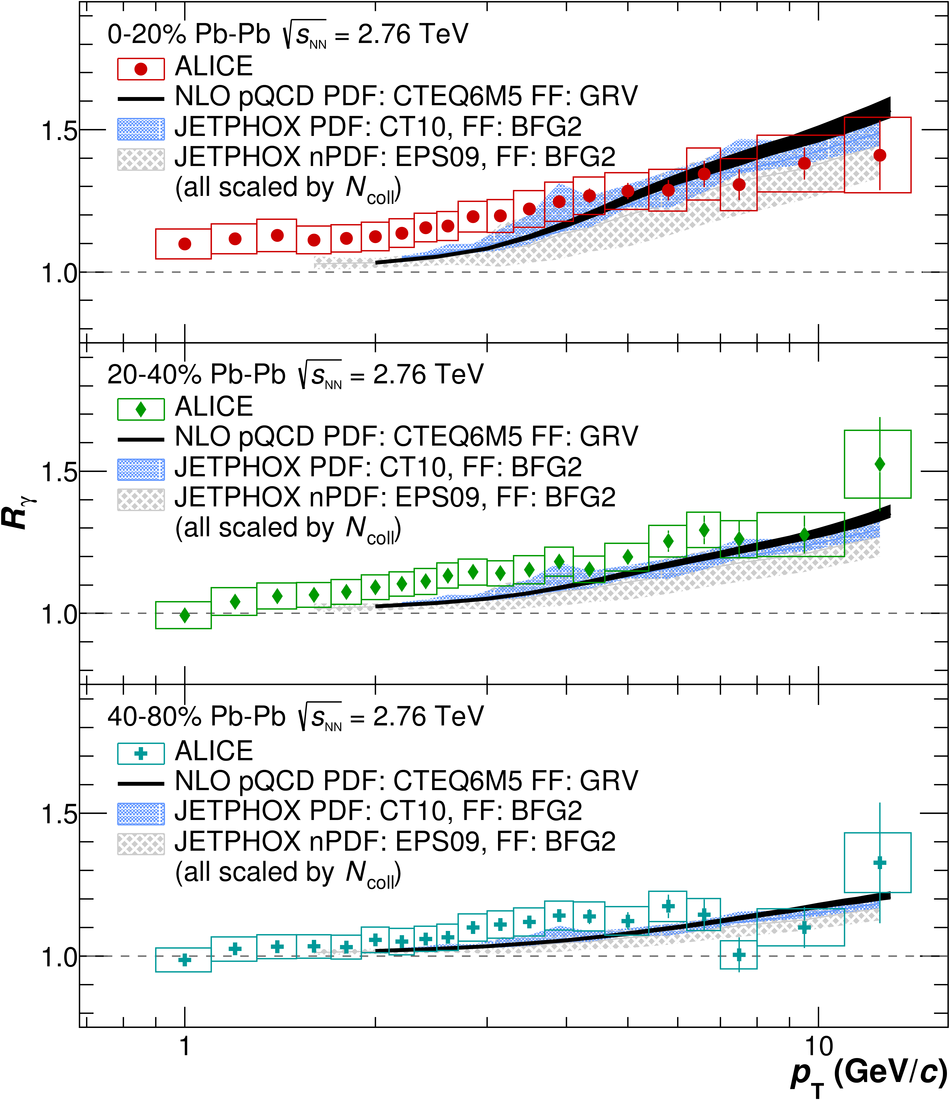
\includegraphics[width=0.45\textwidth]{\main/thermalradiation/figs/RgammaRun1}
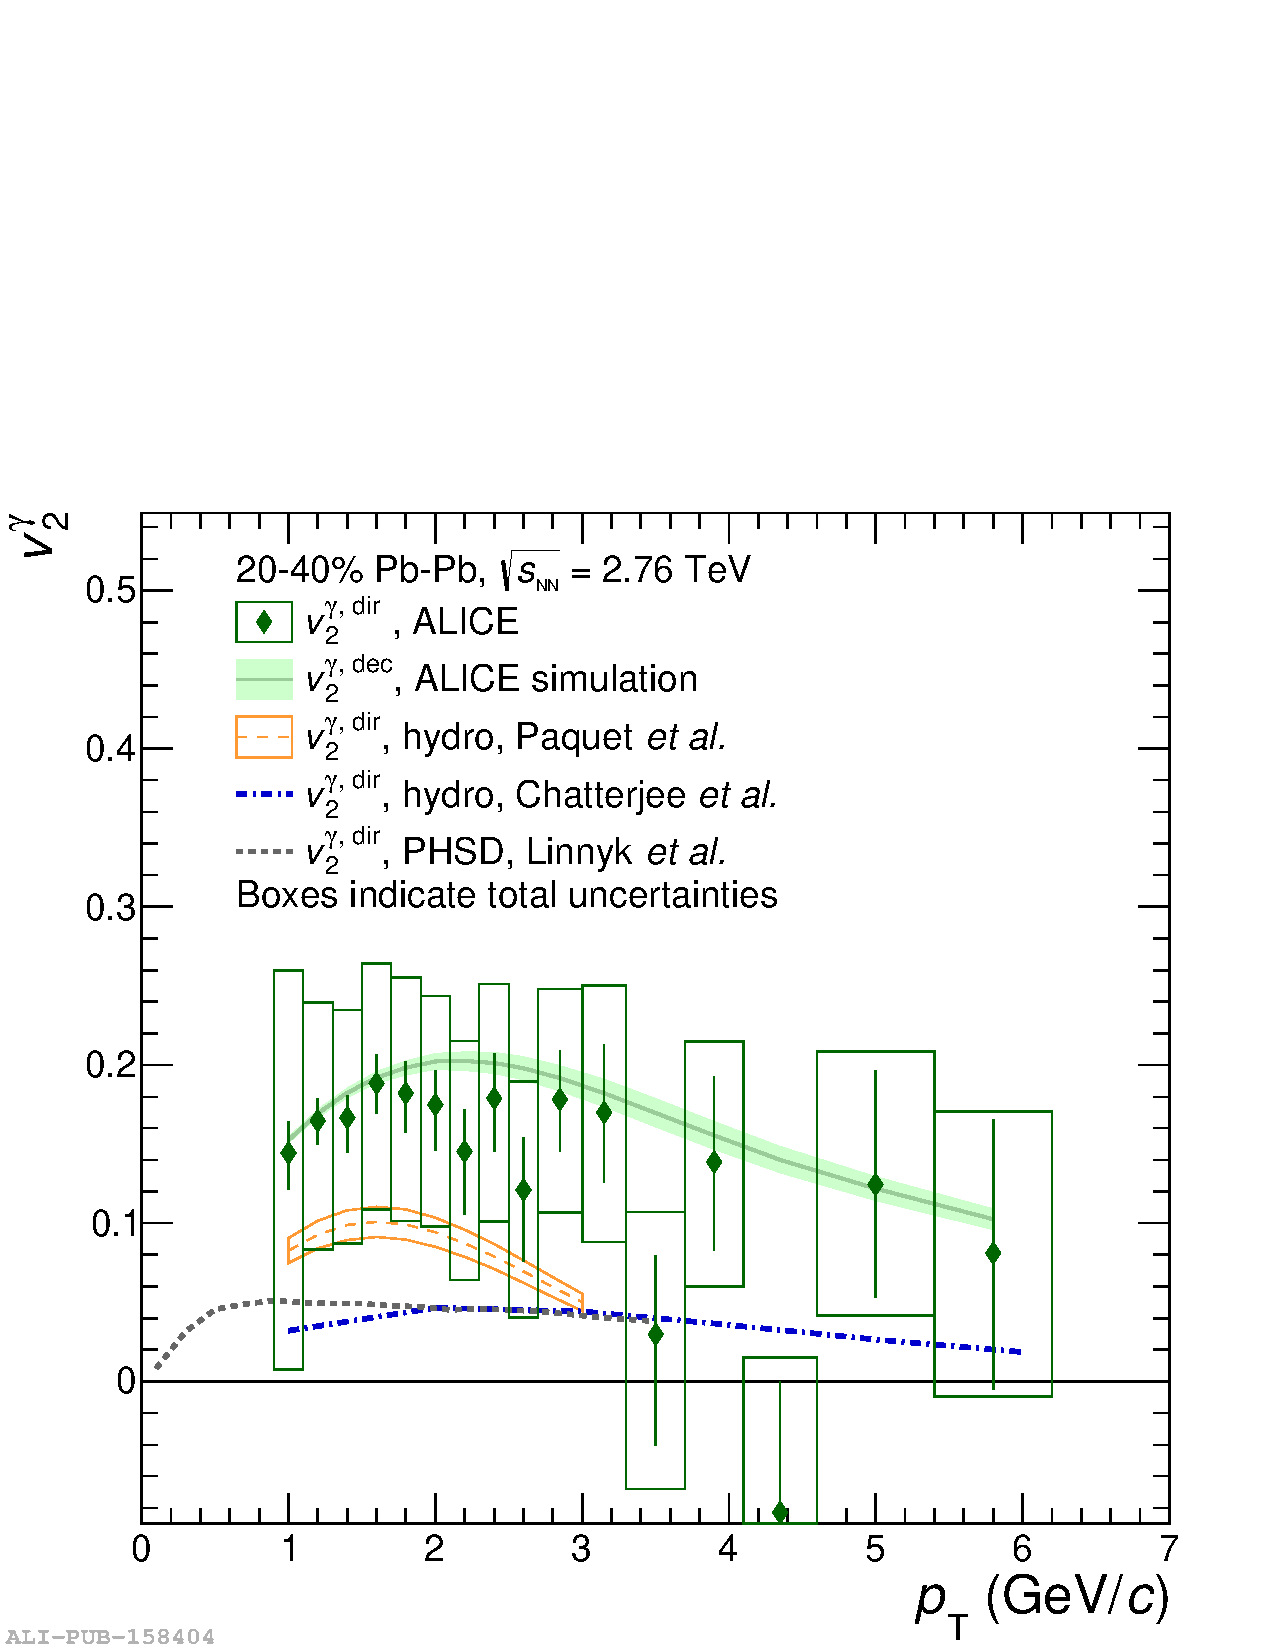
\includegraphics[width=0.45\textwidth]{\main/thermalradiation/figs/2018-May-11-2040_v2dir_combined_theory}
\caption{Placeholder: Measurements of photon spectra ($R_{\gamma}$)}
\label{fig:RealPhotons}
\end{figure}
%-----------------------------------------------------------------------%


\begin{itemize}
\item First measurement at LHC from soft exponential component of photon pT spectrum (ALICE, Phys.Lett. B754 (2016) 235): T ~ 300 MeV (effective temperature averaged over system evolution)
\item "Photon puzzle"
\item Projections for Run3/4 in preparation: reduce systematic error (material budget uncertainty)
\end{itemize}
